\documentclass{beamer}
% \documentclass[aspectratio=169]{beamer}

\usepackage{booktabs}
\usepackage{adjustbox}

\usepackage{pgfplots}
\pgfplotsset{compat=newest}

\pgfplotscreateplotcyclelist{mylist cycle}{%
  {TolDarkBlue, mark=*, mark size=1.5pt},
  {TolLightBrown, mark=square*, mark size=1.3pt},
  {TolLightGreen, mark=triangle*, mark size=1.5pt},
  {TolDarkBrown, mark=diamond*, mark size=1.5pt},
  {TolDarkBlue, mark=star*, mark size=1.5pt},
  {TolLightBrown, mark=otimes*, mark size=1.3pt},
}

\usepackage[utf8]{inputenc}
\usepackage{microtype}

% Beamer Configuration
\usepackage{appendixnumberbeamer}
\hypersetup{pdfstartview={Fit}}
\usetheme{metropolis}

% General Latex configuration
\usepackage[english]{babel}
\usepackage{csquotes}
\usepackage[backend=biber,style=ieee]{biblatex}
\bibliography{./bibliography.bib}	

% Code
\usepackage{xcolor}
\usepackage[outputdir=.texpadtmp,section]{minted}
\definecolor{light-gray}{gray}{0.9}
% \begin{javascriptcode}...
\newminted{javascript}{tabsize=2, linenos=true, fontsize=\scriptsize, xleftmargin=3.5ex, highlightcolor=light-gray}

% \javascript/code/
\newmintinline{javascript}{}

% \javascriptfile{name}
\newmintedfile{javascript}{tabsize=2, linenos=true, fontsize=\scriptsize, xleftmargin=3.5ex, mathescape,  breaklines=true}

% Presentation configuration
\author{Micha Reiser}
\title{Parallel.es}
\subtitle{Parallelize your JavaScript Applications with Ease}
\institute{HSR}

\titlegraphic{
\includegraphics[width=2cm]{kw_logo}}

\date{\today}

\begin{document}

\begin{frame}
	\maketitle
\end{frame}

\begin{frame}{Overview}
	\tableofcontents
\end{frame}


\section{Motivation}

\begin{frame}[fragile]{Motivation for Parallelization}
	\begin{itemize}[<+->]
		\item Performance
		\item \dots but moreover, a better user experience
	\end{itemize}
\end{frame}

\begin{frame}{A better User Experience?}
	\begin{itemize}
		\item Because JavaScript is single threaded
		\item Long running tasks are blocking the UI-thread
		\item and therefore, the UI is not responsive
	\end{itemize}
\end{frame}

\begin{frame}{The JavaScript Event Loop is the Reason therefore}
	\begin{center}
		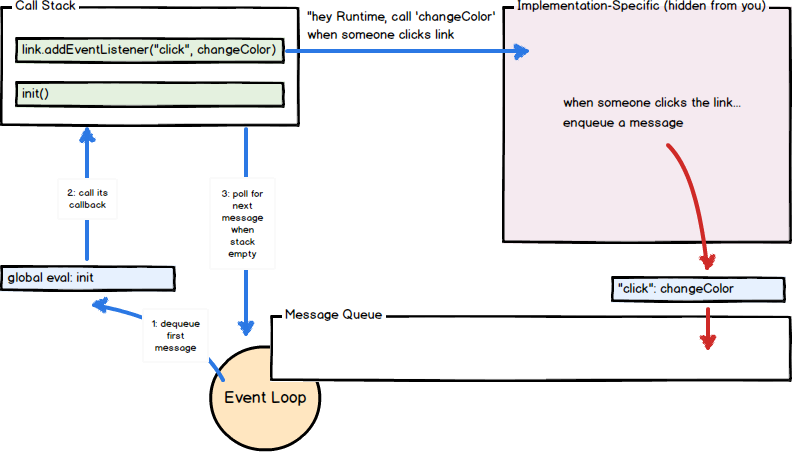
\includegraphics[width=0.9\textwidth]{event-loop}\cite{Swenson-Healey2013}
	\end{center}
\end{frame}


\section{Initial Position}

\begin{frame}{Technologies offered by the Runtime Environment}
	\begin{itemize}
		\item Browser: Web Worker Standard~\cite{w3cWebWorker}
		\item Node: Child Process~\cite{childProcess}
		\item JVM: RingoJS~\cite{RingoJS}
	\end{itemize}
\end{frame}

\begin{frame}{Web Worker Architecture}
	\begin{center}
		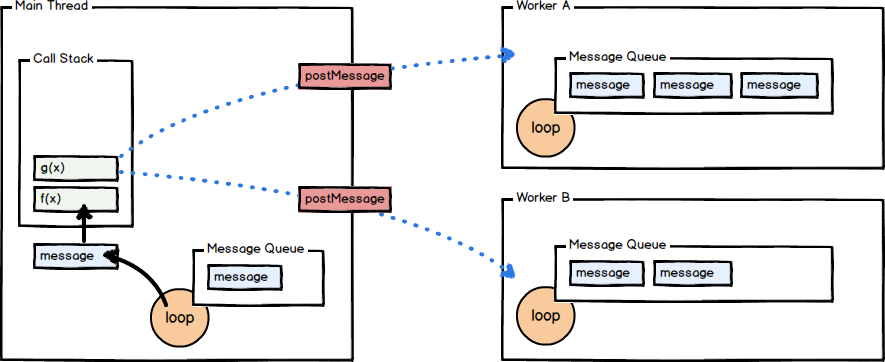
\includegraphics[width=0.9\textwidth]{web-workers}~\cite{Swenson-Healey2013}
	\end{center}
	
	\begin{alertblock}{Memory}
		Each Web Worker uses a distinct runtime environment (e.g. V8), therefore, the memory of each web worker is distinct too.
	\end{alertblock}

\end{frame}

\begin{frame}[fragile]{\enquote{Simple} Web Worker Example}
	\begin{columns}[t]
		\begin{column}{0.56\textwidth}
			\begin{block}{main.js}
				\begin{javascriptcode}
const worker = new Worker("./worker.js");
worker.postMessage(40);

worker.addEventListener(
	"message", 
	result => console.log(result.data)
);
				\end{javascriptcode}
			\end{block}
		\end{column}
		\pause
		\begin{column}{0.44\textwidth}
			\begin{block}{worker.js}
				\begin{javascriptcode}
function fib(num) {
	if(num <= 2) {
		return 1;
	}
	return fib(num - 1) + 
		fib(num - 2);
}

onmessage = function (event) {
	const num = event.data;
	const result = fib(num);
	postMessage({ 
		number: num, 
		fib: result 
	});
};	
				\end{javascriptcode}
			\end{block}
		\end{column}

	\end{columns}

\end{frame}

\begin{frame}{But I also have to\dots}
	\begin{itemize}
		\item Handle Errors 
		\item Return a Promise in the UI-Thread
		\item Perform the Computation for multiple Items
		\item Besides, it should run on Node.JS too
	\end{itemize}
\end{frame}

\begin{frame}{And I don't like that\dots}
	\begin{itemize}
		\item code splitting is enforced by technology instead of by semantics
		\item the messaging model results in a clear seam 
		\item integration adds non inherent complexity
		\item the build gets far more complicated
	\end{itemize}
\end{frame}
\section{Parallel.es}
\subsection{Overview}

\begin{frame}{Parallel.es eases parallelizing JavaScript applications}
	\begin{itemize}
		\item The API is type-safe
		\item \dots and runtime environment independent, write once, run everywhere
		\item Uses a thread pool
		\item Detects the optimum of threads to create
	\end{itemize}
\end{frame}

\begin{frame}[fragile]{\enquote{Simple} Example}
	\begin{javascriptcode}
import parallel from "parallel-es";

function fib(num) {
	if(num <= 2) {
		return 1;
	}
	return fib(num - 1) + fib(num - 2);
}

parallel.run(fib, 40)
	.catch(error => console.error(error))
	.then(result => console.log(result));
	\end{javascriptcode}
\end{frame}

\begin{frame}{The Mandelbrot Showcase}
	\begin{center}
		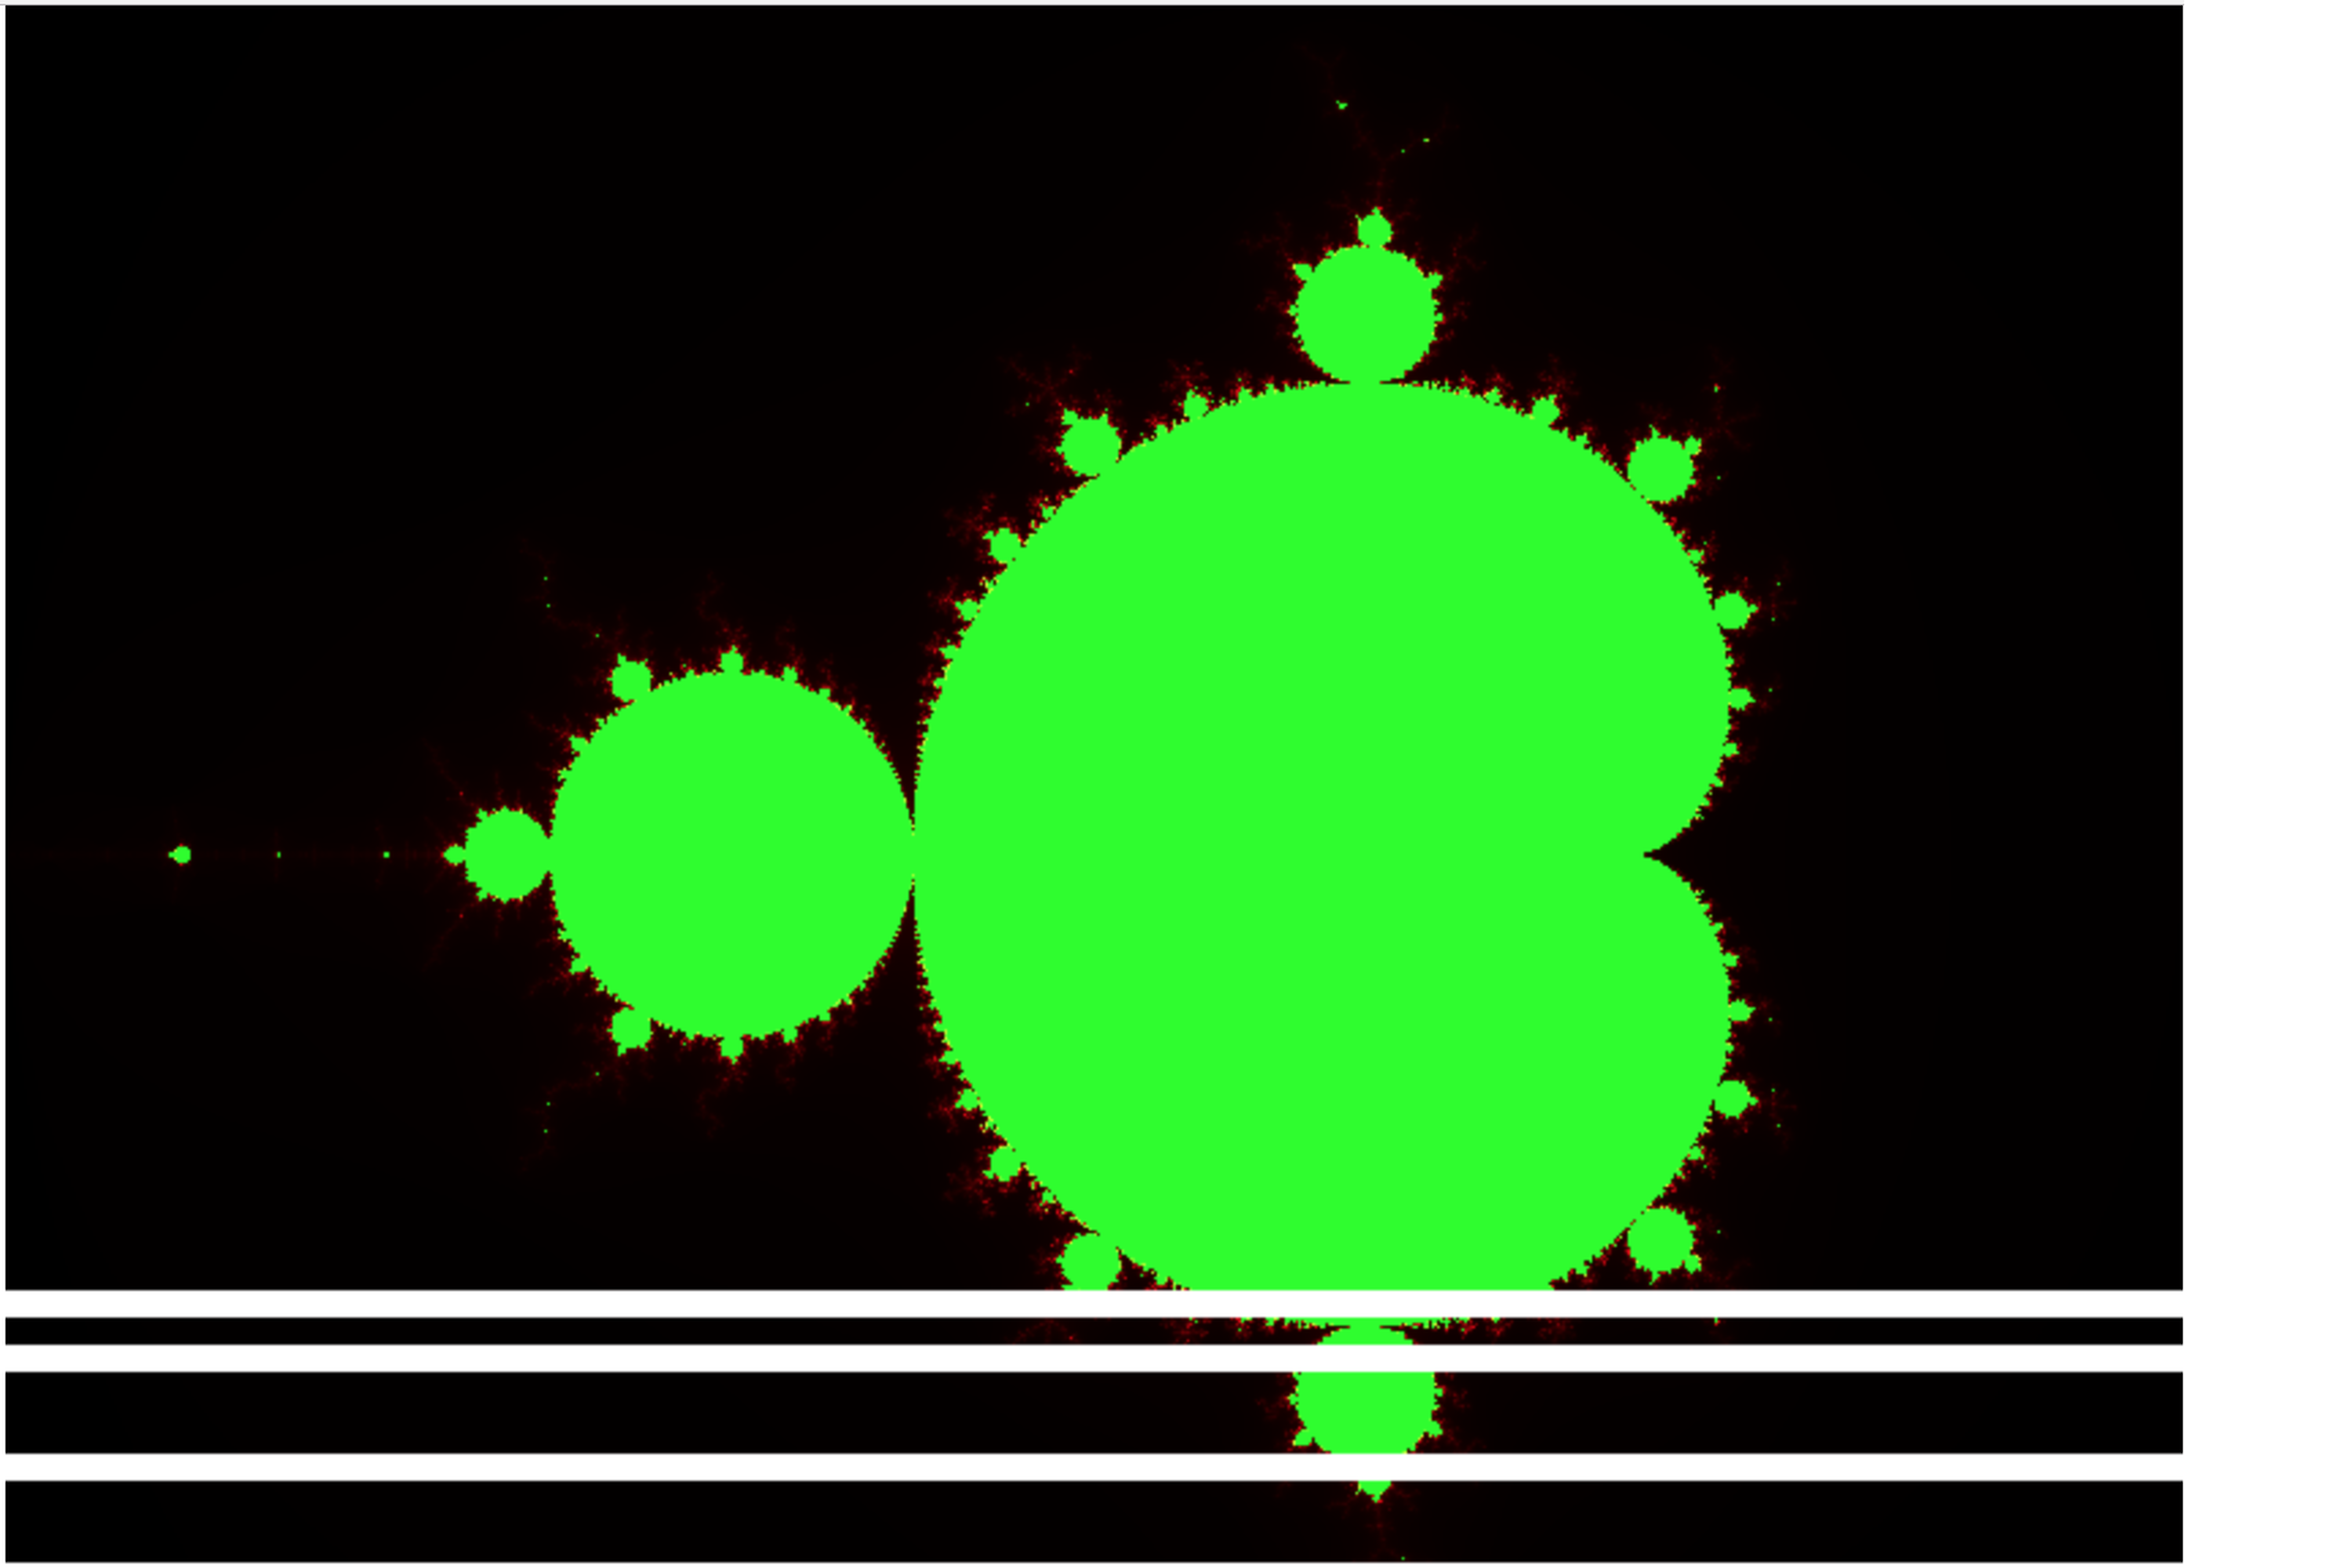
\includegraphics[height=0.7\textheight]{mandelbrot}
	\end{center}
	
	\url{https://michareiser.github.io/parallel-es-example/}
\end{frame}

\begin{frame}[fragile, shrink]{Code for Single Threaded Execution}
		\begin{javascriptcode}
const imageWidth = 10000;
const imageHeight = 10000;

function computePixel(x, y) {
	// ...
	return n;
}

function computeMandelbrotLine(y) {
	const line = new Uint8ClampedArray(imageWidth * 4);
	for (let x = 0; x < imageWidth; ++x) {
		line[x * 4] = computePixel(x, y);
	}
	return line;
}

const result = _.chain()
	.range(imageHeight)
	.map(computeMandelbrotLine)
	.value();
	
// draw to canvas
\end{javascriptcode}
\end{frame}

\begin{frame}{Idea}
	\begin{itemize}
		\item Compute Lines in Background Threads
		\item Preferred, create as many Background Threads as CPU's are available
	\end{itemize}
\end{frame}

\begin{frame}[fragile]{Poor Mans Solution}
	\begin{javascriptcode}
const imageWidth = 10000;
const imageHeight = 10000;

function computePixel(x, y) {
	// ...
	return n;
}

function computeMandelbrotLine(y) {
	// ...
	return line;
}

for (int i = 0; i < imageHeight; ++i) {
	parallel.run(computeMandelbrotLine, i).then(line => {
		// draw to canvas
	});
}
	\end{javascriptcode}
\end{frame}

\begin{frame}{It works\footnote{Actually, it depends, details follow}! But\dots}
	\begin{itemize}
		\item I don't want to be responsible to split the work on multiple threads
		\item Flow of logic is hard to catch
	\end{itemize}
\end{frame}

\begin{frame}{Therefore, Parallel.es offers a descriptive API}
	\begin{itemize}
		\item Inspired by lodash / underscore
		\item Handles Work Partitioning
		\item Allows subscribing to sub results
		\item \dots or the joined overall result
	\end{itemize}
\end{frame}

\begin{frame}[fragile, shrink]{Descriptive Implementation}
\begin{javascriptcode}
const imageWidth = 10000;
const imageHeight = 10000;

function computePixel(x, y) {
	// ...
	return n;
}

function computeMandelbrotLine(y) {
	const line = new Uint8ClampedArray(imageWidth * 4);
	for (let x = 0; x < imageWidth; ++x) {
		line[x * 4] = computePixel(x, y);
	}
	return line;
}

parallel
	.range(imageHeight) 
	.map(computeMandelbrotLine)	 
	.subscribe((subResult, index, batchSize) => /* draw line */)
	.catch(error => /* handle error in computation of any line */)
	.then(result => /* handle overall result */);
	\end{javascriptcode}
\end{frame}

\subsection{Implementation}

\begin{frame}{Difficulties}
	Each Worker has its distinct memory and therefore, 
	\begin{itemize}
		\item data needs to be transferred between workers
		\item \dots as well as all functions executed in background threads
	\end{itemize}
	
	\vfill
	
	\begin{block}{Comparsion to other Languages}
		Other languages, e.g. Java, have a shared memory that is accessible by all threads. However, 
			parallelization in JavaScript is more like multiprocess programming using inter process communication.
	\end{block}
\end{frame}

\begin{frame}{Two Possibilities}
	\begin{itemize}
		\item Runtime Serialization of Functions
		\item Transpilation of Source Code
	\end{itemize}
\end{frame}

\begin{frame}{Runtime Serialization of Functions - Overview}
	\begin{center}
		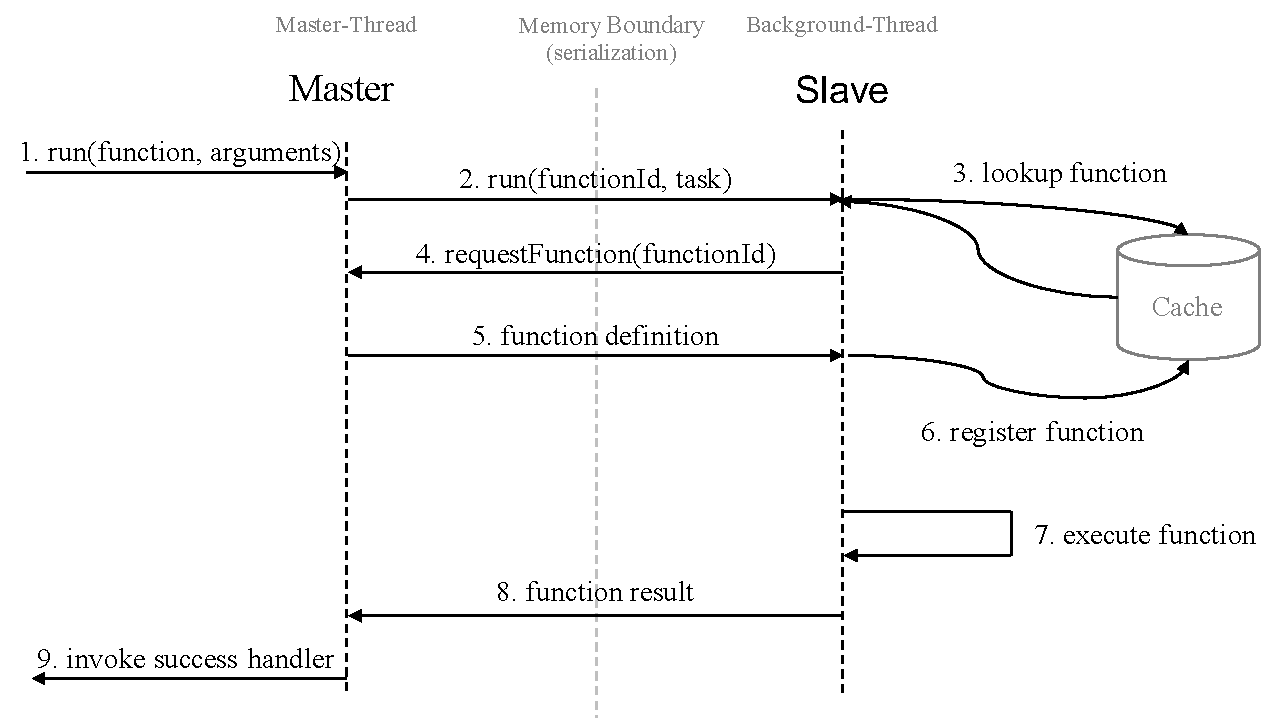
\includegraphics[width=0.8\textwidth]{runtime-system}
	\end{center}
\end{frame}

\begin{frame}[fragile, shrink]{Runtime Serialization of Functions - Serialization}
	\begin{javascriptcode}
const s = func.toString();
const name = getFunctionName(func);
const args = s.substring(s.indexOf("(") + 1, s.indexOf(")")).split(",");
const body = s.substring(s.indexOf("{") + 1, s.lastIndexOf("}")).trim();

const definition = {
	argumentNames: args.map(arg => arg.trim()),
	body,
	id,
	name: name ? name : undefined
};
\end{javascriptcode}

\end{frame}

\begin{frame}[fragile, shrink]{Runtime Serialization of Functions - Deserialization}
	\begin{javascriptcode}
if (definition.name) {
	const args = definition.argumentNames.join(", ");
	const source = `return function ${definition.name} (${args}) { 
		${definition.body} 
	};`; 
	const wrapper = Function.apply(undefined, [ source ]);
	return wrapper();
}
	
return Function.apply(undefined, [
	...definition.argumentNames, 
	definition.body
]);	
\end{javascriptcode}
\end{frame}

\begin{frame}{But what about a Function's Closure?}
\begin{itemize}
	\item Transitive Functions
	\item \dots or Variables referenced from the Function's outer Scope
\end{itemize}

are not supported by Runtime Serialization

\vfill 

\begin{block}{Why Not?}
It's possible to analyze a function at runtime, e.g. by using Babel. However, there is no way to get access to the values of a function's closure as it is the case in C\#. 	
\end{block}
\end{frame}

\begin{frame}[fragile, shrink]{The Issue with Function Closures and Runtime Serialization}
	\begin{columns}[t]
	\begin{column}{0.5\textwidth}
		\begin{block}{UI-Thread}
		\begin{javascriptcode*}{highlightlines={9, 11}, fontsize=\tiny}
const width = 10000;
const height = 10000;

function computePixel(x, y) {
	// ...
}

function computeMandelbrotLine(y) {
	const l = new Uint8ClampedArray(width * 4);
	for (let x = 0; x < width; ++x) {
		l[x * 4] = computePixel(x, y);
	}
	return l;
}

parallel
	.range(height) 
	.map(computeMandelbrotLine)	 
	.then(result => /* handle overall result */);
	\end{javascriptcode*}
	\end{block}
	\end{column}
	\pause
	\begin{column}{0.5\textwidth}
		\begin{block}{Worker-Thread}
			\begin{javascriptcode*}{fontsize=\tiny, highlightlines={2, 4}}
function computeMandelbrotLine(y) {
	const l = new Uint8ClampedArray(width * 4);
	for (let x = 0; x < width; ++x) {
		l[x * 4] = computePixel(x, y);
	}
	return l;
}	
			\end{javascriptcode*}

		\end{block}
		
		\begin{alertblock}{Issue}
			\javascriptinline/height/ variable and \javascriptinline/computePixel/ function are not defined in worker-thread.
		\end{alertblock}
	\end{column}
\end{columns}
\end{frame}

\begin{frame}{Source Code Transpilation}
	\begin{itemize}
		\item Analyses all calls to \javascriptinline/parallel/
		\item Extracts passed functions 
		\item \dots and as well transitive functions
		\item Registers these functions in the background-thread source file
		\item Split into a Babel (extraction) and Webpack-Plugin (registration)
	\end{itemize}
\end{frame}

\begin{frame}[fragile, shrink]{Transpiled Code of Mandelbrot Example}
\begin{columns}[t]
	\begin{column}{0.5\textwidth}
		UI-Thread
		\begin{javascriptcode*}{highlightlines={8-10, 20-24}, fontsize=\tiny}
const width = 10000;
const height = 10000;

function computePixel(x, y) {
	// ...
}

function _environmentExtractor() { 
	return { width: width };
}

function computeMandelbrotLine(y) {
	const l = new Uint8ClampedArray(width * 4);
	// ...
	return l;
}

parallel
	.range(height)
	.inEnvironment(_environmentExtractor()) 
	.map({ 
		identifier: "static:_entrycomputeMandelbrotLine",
		_______isFunctionId: true
	}) 
	.then(result => console.log(result));
\end{javascriptcode*}
	\end{column}
	\begin{column}{0.5\textwidth}
	Worker-Thread
	\begin{javascriptcode*}{highlightlines={1, 2, 6, 12, 22-27}, fontsize=\tiny}
var width;
function computePixel(x, y) { 
	// ...
}

function computeMandelbrotLine(y) { 
	var l = new Uint8ClampedArray(width * 4);
	// ..
	return l;
}
 
function _entrycomputeMandelbrotLine() { 
	try {
		var _environment = arguments[arguments.length - 1];
		width = _environment.width; 
		return computeMandelbrotLine.apply(this, arguments); 
	} finally {
		width = undefined;
	}
} 

slaveFunctionLookupTable.registerStaticFunction({
		identifier: 'static:_entrycomputeMandelbrotLine',
		_______isFunctionId: true
	}, _entrycomputeMandelbrotLine);
\end{javascriptcode*}
	\end{column}
\end{columns}


\end{frame}
\section{Use Case}
\begin{frame}{Riskprofiling}
	\begin{center}
		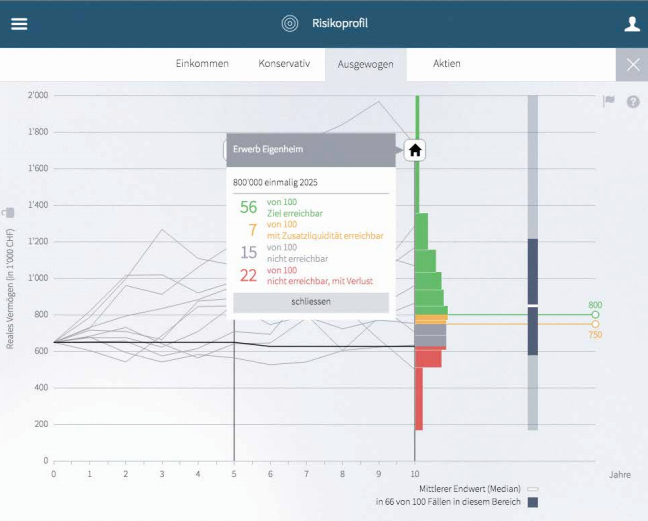
\includegraphics[width=0.8\textwidth]{risk-profiling}
	\end{center}
\end{frame}

\begin{frame}{Performance Improving prior Parallelization}
	\begin{itemize}
		\item A problem needs to be parallelizable
		\item Parallelization always adds complexity
		\item Maybe it's enough to improve \enquote{synchronous} code
	\end{itemize}
\end{frame}

\begin{frame}[plain]
	\begin{tikzpicture}
		\begin{axis}[
			mlineplot,
			width=1\textwidth,
			height=1\textheight,
			title=Execution Time for 100'000 runs,
			xlabel={Projects},
			ylabel={Mean in seconds},
			xmin=0,
			xmax=18,
			xtick={1, 4, 8, 16},
			ymin=0,
			ymax=2.8,
			legend entries={v1,v2,v3, v4, v5, v6, v7},
			legend style = { at = {(0.2,1.0)}},
			minor tick num=5,
			cycle list name=mylist cycle
		]
		\addplot table {../v1.data};
		\addplot table {../v2.data};
		\addplot table {../v3.data};
		\addplot table {../v4.data};
		\addplot table {../v5.data};
		\addplot table {../v6.data};
		\addplot table {../v7.data};
	\end{axis}
\end{tikzpicture}
\end{frame}

\begin{frame}{V1, authored by Micha Reiser}
	\begin{itemize}
		\item Computes the simulation result over 15 years
		\item For each project
		\begin{itemize}
			\item Creates the four groups \enquote{red, gray, yellow, green}
			\item Creates for each group 10 buckets and assigns the simulation values
		\end{itemize}
		\item Median, min, max are computed in the chart
	\end{itemize}
	
	\begin{alertblock}{Main Concern}
		Simulation returns all values instead of the needed information median, min and max. Therefore, absolutely unsuited for parallelization because of large data amount to be transferred.
	\end{alertblock}

\end{frame}

\begin{frame}{V2, only returns Information needed by Chart}
	\begin{itemize}
		\item Marginal Faster (no array resizes, $\approx 20$ms)
		\item Chart needs to perform less computations
		\item Easier to parallelize, less data needs to be transferred
	\end{itemize}
\end{frame}

\begin{frame}{V3, Address V8 deoptimizations}
	If you see this...
	
	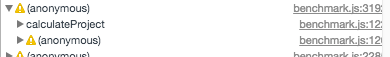
\includegraphics[scale=0.45]{deopt}
	
	... you are doomed ;)
\end{frame}

\begin{frame}{...or at least, there is much Room for Improvements}
	\begin{block}{V8 Optimization Killers~\cite{bluebird2017}}
		\begin{itemize}
			\item Unsupported Syntax (e.g. \javascriptinline/debugger/, \javascriptinline/eval/, \javascriptinline/with/, generator functions...) 
			\item Manipulating \javascriptinline/arguments/
			\item Very large Switch-case Statements (+128 cases)
			\item \javascriptinline/for in/
			\item Infinite Loops with deep logic or unclear exit
			\item Others
		\end{itemize}
	\end{block}
	
	\pause
	\begin{block}{Workaround}
		\begin{itemize}
			\item Clean Code
			\item Small Functions
		\end{itemize}	
	\end{block}
\end{frame}

\begin{frame}[fragile, shrink]{In this Case, the Reason is a Dynamic Object Structure}
	\begin{javascriptcode*}{highlightlines={18-20}, fontsize=\tiny}
const valuesByGroup: { [groupName: string]: number } = {};
const bucketSize = Math.round(simulatedValuesThisYear.length / NUMBER_OF_BUCKETS);
const buckets: IBucket[] = [];

for (let i = 0; i < simulatedValuesThisYear.length; i += bucketSize) {
	const bucket: IBucket = {
		max: Number.MIN_VALUE,
		min: Number.MAX_VALUE,
		subBuckets: {}
	};

	for (let j = i; j < i + bucketSize; ++j) {
		const value = simulatedValuesThisYear[j];
		bucket.min = Math.min(bucket.min, value);
		bucket.max = Math.max(bucket.max, value);

		const group = groupForValue(simulatedValuesThisYear[j], groups);
		valuesByGroup[group.name] = (valuesByGroup[group.name] || 0) + 1;
		const subBucket = bucket.subBuckets[group.name] = bucket.subBuckets[group.name] || 
						{ group: group.name, max: Number.MIN_VALUE, min: Number.MAX_VALUE };
		subBucket.min = Math.min(subBucket.min, value);
		subBucket.max = Math.max(subBucket.max, value);
	}

	buckets.push(bucket);
}
	\end{javascriptcode*}

\end{frame}

\begin{frame}{...that makes it Impossible to Optimize the Property Access}
	\begin{center}
		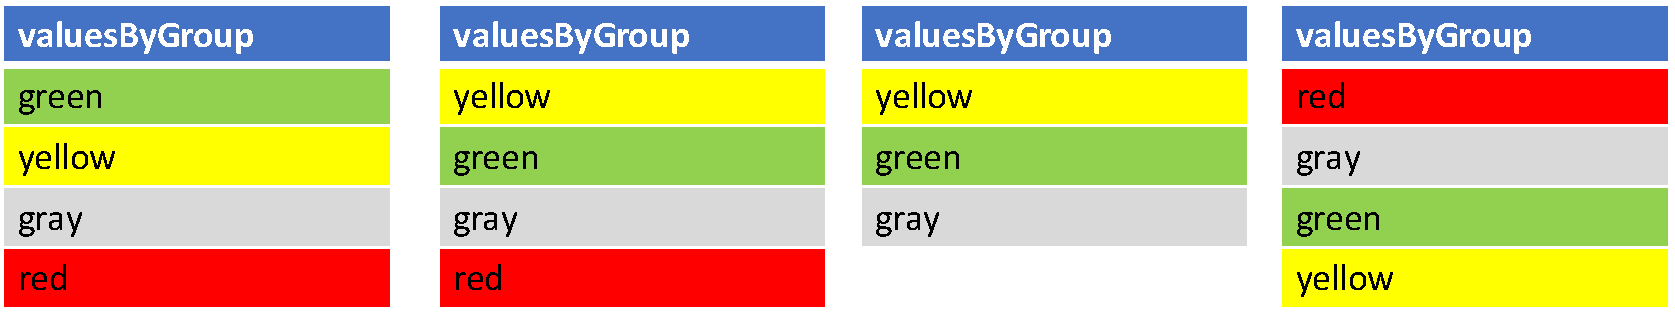
\includegraphics[width=1\textwidth]{memory-model}
	\end{center}
	
	Depending on the order of the simulated values the offset for the properties differ, e.g. for \enquote{green}:
	
	\begin{enumerate}[<+->]
		\item +0
		\item +4 (32bit pointer)
		\item +4
		\item +8
		\item ...
	\end{enumerate}
	
	\only<6>{Therefore, V8 deoptimizes the \textbf{whole} function}
\end{frame}

\begin{frame}[fragile, shrink]{Solution: Ensure that the Object is always Initialized in the same Order}
	\begin{javascriptcode}
const bucket: IBucket = {
	max: Number.MIN_SAFE_INTEGER,
	min: Number.MAX_SAFE_INTEGER,
	// Needed to avoid deoptimization because of changed attribute orders in subBuckets. Initialize with const order
	subBuckets: {
		green: {
			group: "green",
			max: Number.MIN_SAFE_INTEGER,
			min: Number.MAX_SAFE_INTEGER,
			empty: true
		},
		yellow: {
			group: "yellow",
			max: Number.MIN_SAFE_INTEGER,
			min: Number.MAX_SAFE_INTEGER,
			empty: true
		},
		//...
	}
};	
	\end{javascriptcode}
\end{frame}

\begin{frame}{This small Change Improves Performance by up to 235ms}
	\begin{tikzpicture}
		\begin{axis}[
			mlineplot,
			width=1\textwidth,
			height=1\textheight,
			title=Execution Time for 100'000 runs,
			xlabel={Projects},
			ylabel={Mean in seconds},
			xmin=0,
			xmax=18,
			xtick={1, 4, 8, 16},
			ymin=0,
			ymax=2.8,
			legend entries={v1,v3},
			legend style = { at = {(0.2,1.0)}},
			minor tick num=5,
			cycle list name=mylist cycle
		]
		\addplot table {../v1.data};
		\addplot table {../v3.data};
	\end{axis}
\end{tikzpicture}
\end{frame}

\begin{frame}{Further Improvements}
	\begin{itemize}
		\item v4: Reduce Nesting of Functions (-47ms)
		\item v5: Create Arrays with expected Size (-60ms)
		\item v6: Only simulate number of Years needed (-270ms)
		\item v7: Avoid Object Destructuring (-61ms)
	\end{itemize}
	
	\begin{block}{Overall}
		Improvement by 666ms in best case (1.76 instead of 2.426s) or by 28\%
	\end{block}

\end{frame}

\begin{frame}{Further Improving the Performance by Parallelizing the Computation}
	\begin{itemize}[<+->]
		\item Computation consists of
			\begin{itemize}
				\item Simulation
				\item Creating Buckets for each Projects
			\end{itemize}
		\item Parallelization by computing buckets for multiple projects simultaneous 
		\item However, simulation is most expensive
		\item But sharing the data of the simulation between worker is as expensive as performing the simulation in each worker
		\item So it only makes sense to parallelize if there are 2+ projects
	\end{itemize}
	
	\only<8>{\begin{block}{But Performance is not everyting}
		The UI is no longer blocked for $\approx 2$s
	\end{block}}

\end{frame}

\begin{frame}{Performance Improvement of up to 300ms (2 Cores, HT)}
	\begin{tikzpicture}
		\begin{axis}[
			mlineplot,
			width=1\textwidth,
			height=0.8\textheight,
			title=Execution Time for 100'000 runs,
			xlabel={Projects},
			ylabel={Mean in seconds},
			xmin=0,
			xmax=18,
			xtick={1, 4, 8, 16},
			ymin=0,
			ymax=2.8,
			legend entries={v1,v7, transpiled},
			legend style = { at = {(0.3,1.0)}},
			minor tick num=5,
			cycle list name=mylist cycle
		]
		\addplot table {../v1.data};
		\addplot table {../v7.data};
		\addplot table {../transpiled.data};
	\end{axis}
\end{tikzpicture}

But sometimes it is even slower.

\end{frame}

\section{Conclusion}
\begin{frame}{Conclusion}
	\begin{itemize}
		\item Parallel.es eases writing multithreaded JS applications
		\item It is platform independent
		\item Compared to alternatives (\cite{hamstersjs,SavitzkyMayr2016, Wermke2016}), 
		\begin{itemize}
			\item The API is type-safe
			\item Performs well in most cases
			\item Transpilation allows a seamless integration
		\end{itemize}
		\item Source Map support is helpful
		\item However, no support for
			\begin{itemize}
				\item Low Level synchronization primitives
				\item Recursive Tasks
			\end{itemize}
	\end{itemize}
\end{frame}

\begin{frame}{However}
	\begin{itemize}[<+->]
		\item The problem needs to fit to be easy parallelizable
		\item \dots otherwise, a lot of prior work might be needed
		\item \dots maybe, these improvements are already sufficient
		\item \dots and parallelization always adds non-inherent complexity 
	\end{itemize}
\end{frame}

\begin{frame}{Further Work}
	\begin{itemize}[<+->]
		\item WebAssembly: A new standard of the Web
		\item Provides a stack machine 
		\item Allows to run C++ code in the browser
		\item However, who wants to write C++ ;)
		\item Controversial Idea: compile a subset of JS to Web Assembly
		\item Hopefully profit from better performance
		\item And if time allows, take benefit of the pthreads API
	\end{itemize}
\end{frame}

\begin{frame}{Further Resources}
	\begin{itemize}
		\item Project Page~\cite{Reiser2017}
		\item Project Thesis Paper~\cite{Reiser2016}
		\item Optimization Killers~\cite{bluebird2017}
	\end{itemize}
\end{frame}

\begin{frame}[allowframebreaks]{References}
	\printbibliography[heading=none]
\end{frame}


\begin{frame}[standout]
	Questions and Discussion
\end{frame}

\input{appendix}

\end{document}
